\documentclass[11pt]{article}

\usepackage{comment} % enables the use of multi-line comments (\ifx \fi) 
\usepackage[a4paper,margin=1cm]{geometry}
\usepackage[utf8]{inputenc}
\usepackage[ngerman]{isodate}
\usepackage{gensymb}
\usepackage{graphicx}
\usepackage{booktabs}% http://ctan.org/pkg/booktabs
\usepackage{tabularx}
\usepackage{ltablex} % Longtables with tabularx
\usepackage[x11names]{xcolor}
\usepackage{amsmath}
\usepackage{amssymb}
\usepackage{array}
\usepackage{wrapfig}
\usepackage{subcaption}
\usepackage{csquotes}
\usepackage{lscape}
\usepackage{geometry}
\usepackage{multicol}
\usepackage{bm}
\usepackage{enumitem}
\usepackage{hyperref}
\usepackage{mdframed}
\usepackage{scalerel}
\usepackage{stackengine}
\usepackage{mathtools}
\usepackage{pdfpages}

% Code highlighting
\usepackage{minted}
\surroundwithmdframed{minted}

% Be able to caption equations and float them in place
\usepackage{float}

\newmdtheoremenv{theorem}{Theorem}
\geometry{a4paper, margin=2.4cm}

\newcommand\equalhat{\mathrel{\stackon[1.5pt]{=}{\stretchto{\scalerel*[\widthof{=}]{\wedge}{\rule{1ex}{3ex}}}{0.5ex}}}}
\newcommand\defeq{\mathrel{\overset{\makebox[0pt]{\mbox{\normalfont\tiny def}}}{=}}}
\newcolumntype{C}{>{\centering\arraybackslash}X}

\DeclarePairedDelimiter\abs{\lvert}{\rvert}
\DeclarePairedDelimiter\norm{\lVert}{\rVert}

\setcounter{tocdepth}{3}
\setcounter{secnumdepth}{3}

\graphicspath{{./img/}}

\begin{document}
	
\title{Private Law FS20}
\author{Pascal Baumann\\pascal.baumann@stud.hslu.ch}
\maketitle



For errors or improvement raise an issue or make a pull request on the \href{https://github.com/KilnOfTheSecondFlame/mse_summaries}{github repository}.

\tableofcontents
\newpage



\section{Introduction}
The goal of the module is to foster an understanding on the different dimensions of privacy and a thinking in the corresponding contexts. Transferring privacy aspects to
and within the private and work environment and reflecting upon these, establishing links with learning content in the MRU and the technical modules. Acquiring an appreciation of the legal aspects confronting an engineer in demanding professional situations. Gaining awareness in order to avoid damages due to infringements of rights or legal uncertainty. Acquisition of speaking and listening
skills in order to conduct the corresponding specialist discussions with experts.

Law is a social framework, that saves energy by providing an orientation how to manage conflicts and preserve the values of the culture the law was created in. The law legitimises public authorities and courts, and aims to control the power inherent in any system so that no imbalance is present. 

\subsection{Importance of Law in a Technical or Information Technology World}

The law provides a guideline of the allowed/maximum or obligatory requirement/minimum a system has to satisfy. It clarifies obligations, responsibilities and liability. Industry standards apply the law to a specific field, although they do not clear all legal questions most of the time.

In risk management not only technical or organisational risks have to be considered, but also legal measures to mitigate risks. It is prudent to consult legal as soon as possible in a project, otherwise it may be stopped at the last minute and be very costly. By law, management is responsible that an organisation complies to the legal framework.

\subsection{Importance of Privacy and Personal Data Protection}
Personal data in wrong hands may harm the person in question in various forms. Privacy and the \emph{right to forget} is essential in personal development. An owner with a big collection of such personal data gets a lot of power with little oversight or control. One of the main tasks of a state is to protect its citizen, this includes protection from attacks on personal data.

\paragraph{One of the Most Vital Legal Questions}
\begin{theorem}
	{\scriptsize (1)} \textbf{Who} wants from {\scriptsize (2)} \textbf{whom} {\scriptsize (3)}\textbf{what} based on what {\scriptsize (4)}\textbf{title} or right?
\end{theorem}

\begin{figure}[H]
	\centering
	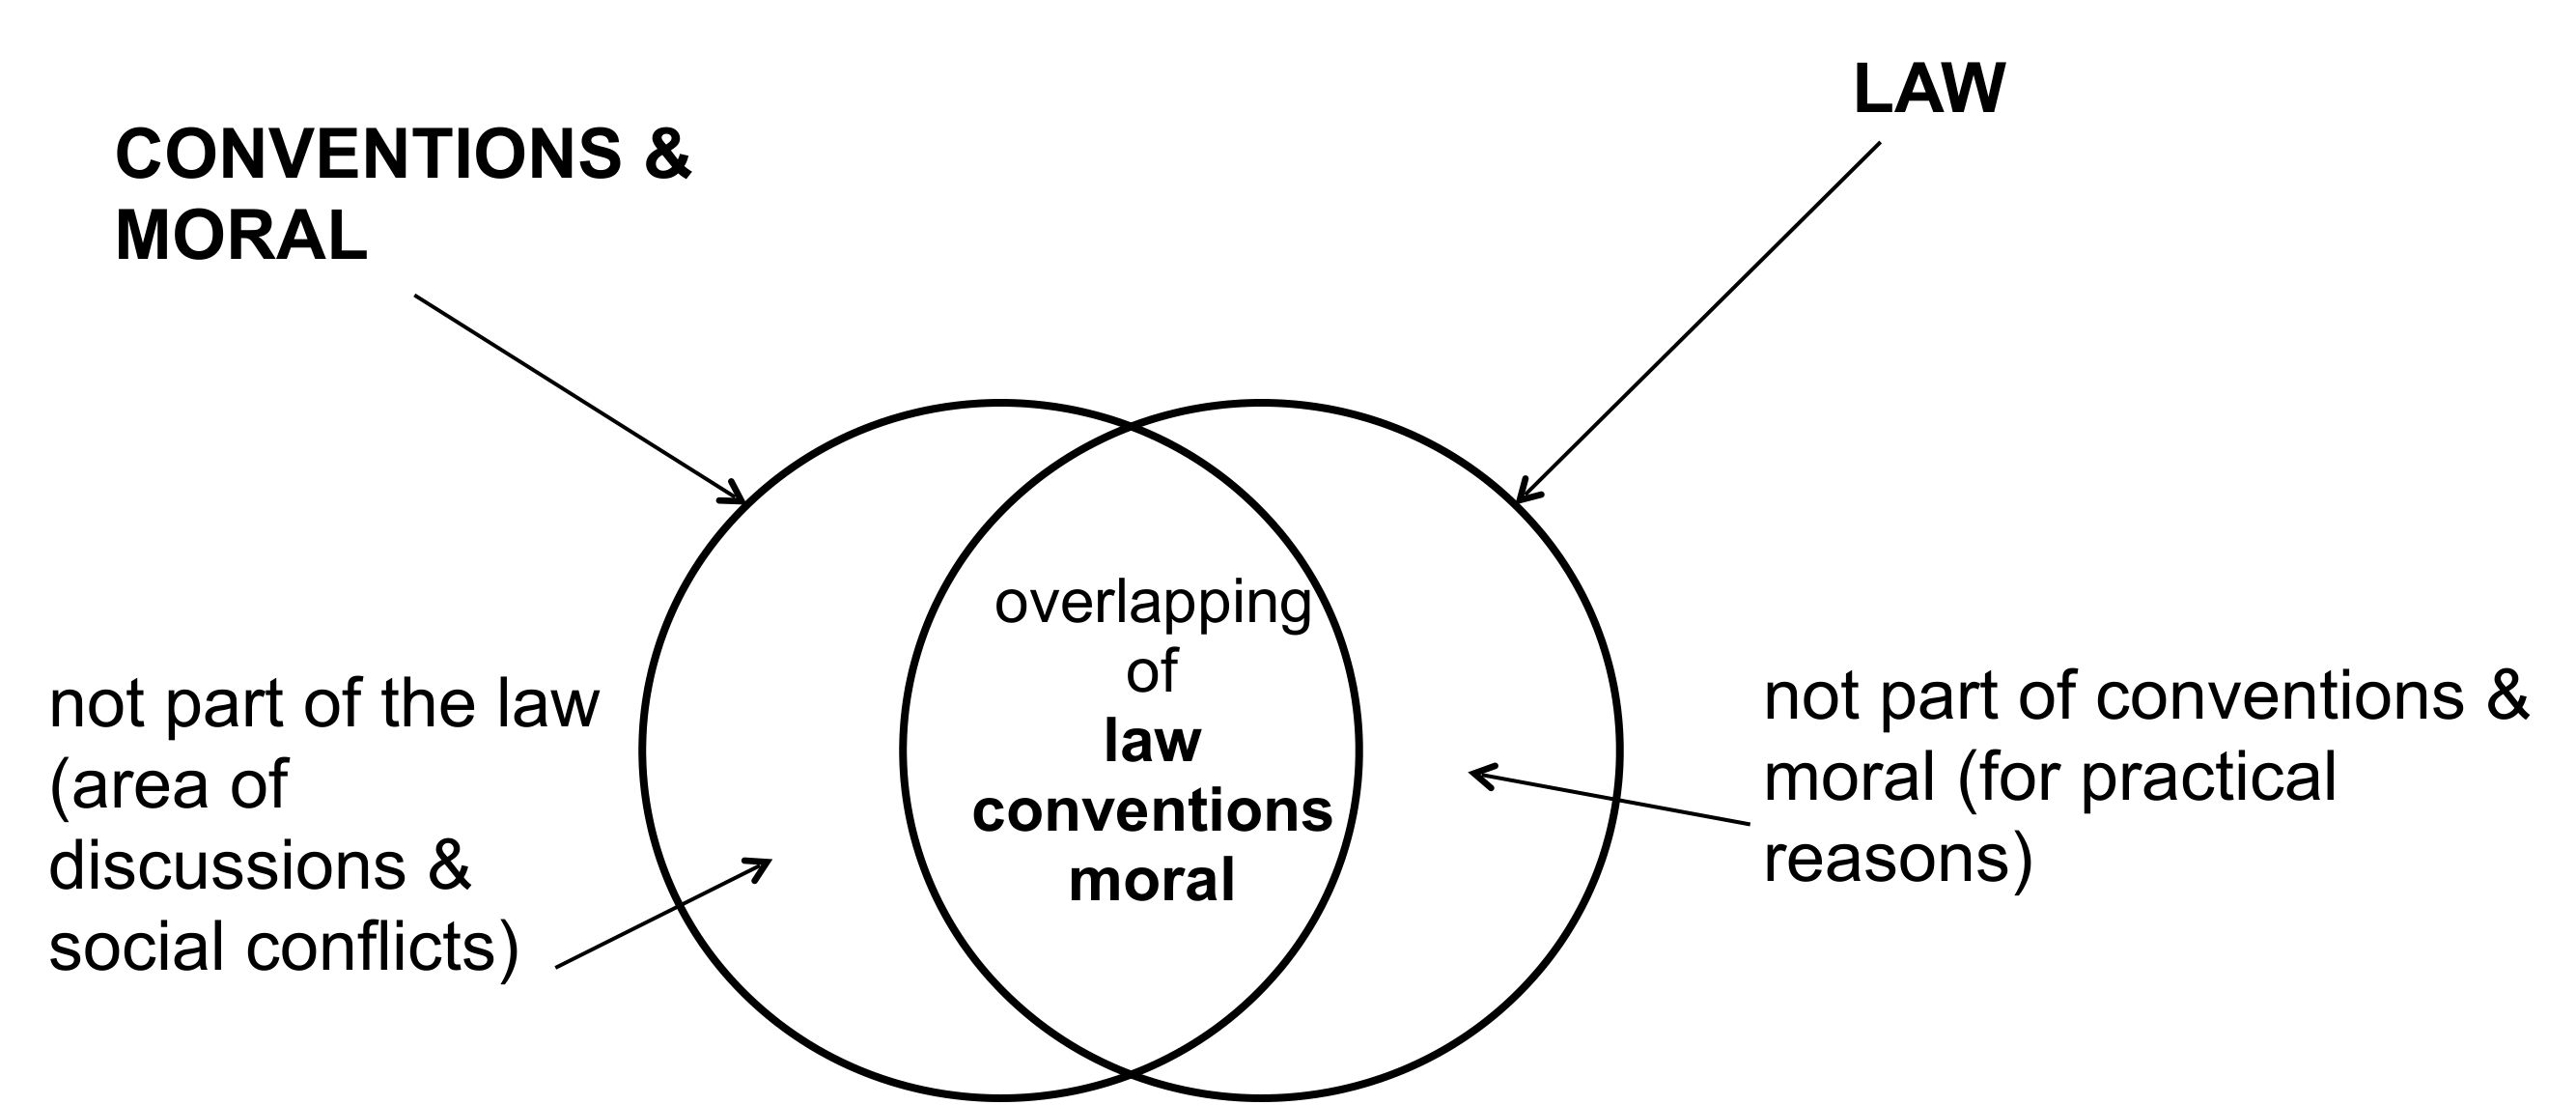
\includegraphics[width=0.8\linewidth]{img/conventions_moral_law}
	\caption{The relationship between conventions, morals and law}
	\label{fig:conventionsmorallaw}
\end{figure}

\subsection{Correct Legal Argumentation}
A statement or claim has to be justified by legal articles or arguments and the necessary evidence. Or is based on legal articles or arguments and with the necessary evidence arrives at a conclusion.

The law get classified by
\begin{itemize}
	\item Status: constitution, act, regulations or by-law
	\item Issuer: Federal, Cantonal and Communal Law
	\item Source of the Law: written law, common law, judicial tradition
	\item Involved Person: Civil Law or Public Law
\end{itemize}

At each of the federal, cantonal and communal level there is a separation of power into the \textbf{legislative}, the \textbf{executive} and the \textbf{Judiciary}, which provides a check and balance on the power of each authority.

\subsection{State, Cantons, Communes}

"Das Schweizervolk und die Kantone [...] bilden die Schweizerische Eidgenossenschaft", (1. Art BV).

"Der Kanton arbeitet mit den Gemeinden, den anderen Kantonen, dem Bund und, in seinem Zuständigkeitsbereich, mit dem Ausland zusammen." Therefore the State is only entitled to legislate and act in a territory or legal field where it has a constitutional legitimacy. The cantons are superior to the state in their power of legislation.

\begin{center}
	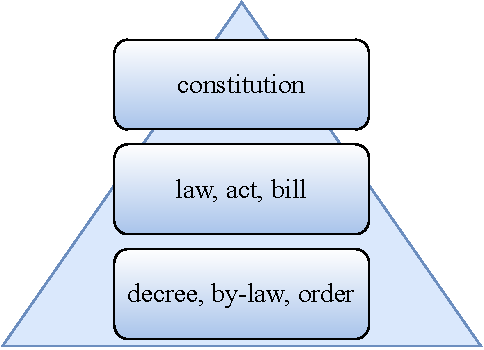
\includegraphics[width=0.4\linewidth,keepaspectratio]{law_hierarchy}
\end{center}

\begin{tabularx}{\linewidth}{X|X}
	\textbf{civil law} & \textbf{public law}\\
	\hline
	OR/ZGB & StGB\\
	GeBüV & FMG\\
	DSG & BÜPF/VÜPF\\
	URG, UWG & EIDI-V\\
	\vdots & \vdots
\end{tabularx}

Civil law is mastered by the \textbf{principle of freedom} of coalition and freedom of contract. Public law is mastered by the \textbf{principle of legality}, the control of power. This results in completely different jurisdictions with different procedures and rights for each.

\subsection{By-Law (Verordnung) $\neq$ Order (Verfügung)}

A By-Law is a \textbf{general, abstract regulation} as part of a law, while an order is an \textbf{individual, concrete application} of a law to a person.

\subsection{Legal Terms}
\begin{itemize}
	\item mandatory rules, stipulated rules and dispositive rules
	\item bona fide or good faith (ZGB 2)
	\item acting in good faith or a fair manner
	\item judicial discretion (ZGB 4)
	\item burden of proof (ZGB 8)
\end{itemize}

\subsection{International Law Framework}
Switzerland is integrated into the European legal framework by long-time traditions, unilateral and bilateral conventions. The IPRG ("Gesetz über das internationale Privatrecht") specifies the bridge between Swiss and foreign law. It rules which law is applicable and which court is competent. Parties can decide in most cases, under which jurisdiction they want to handle their disputes and which court will be competent.

There are generally three different instances in these jurisdictions:
\begin{itemize}
	\item Bezirksgericht
	\item Kantonsgericht
	\item Bundesgericht
\end{itemize}

\end{document}
